%!TEX root = foo-thesis.tex


\chapter{Implementation}

\section{Used Framework and Libraries}

\begin{figure}[htbp]
  \centering
  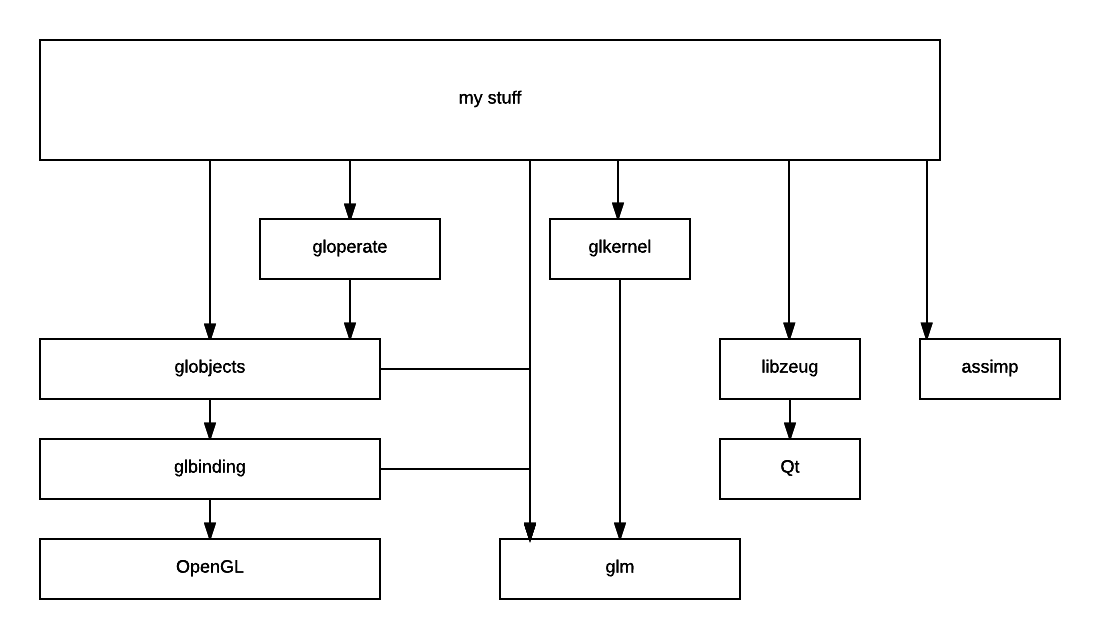
\includegraphics{graphics/Architecture}
  \caption{svg image}
\end{figure}

\begin{outline}
\1 gloperate as framework
    \2 uses qt
\1 libzeug provides GUI elements
\1 globjects as an object-oriented abstraction over OpenGL
\1 glbinding provides OpenGL bindings, directly called sometimes
\1 GLM provides math and easier interaction with the OpenGL API
\1 no further relevance for this thesis:
    \2 assimp for model loading
    \2 glkernel provides kernels for our SSAO implementation
\end{outline}

\section{Rendering Pipeline Overview}
\begin{outline}
\1 would be much the same as the concept pipeline...
\1 show what's compute shader and what not?
\1 it's basically lighting plus
    \2 g-buffer generation
    \2 shadowmap which is part of the RSM,
    \2 SSAO
    \2 deferredshading
    \2 srgb and HDR.
    \2 all of this is not
\1 model loading?
\1 kernel generation?
\end{outline}


\section{RSM Generation and VPL Sampling}
\label{sec:impl:rsmAndVplSampling}
\begin{outline}
\1 use the same code for RSM generation as for G-Buffer generation with only slight modifications:
\1 don't use normalmaps as the triangle normals are sufficient
\1 instead of individual texture lookups, we use the material's average color as diffuse color as suggested by \citet{hedman2016sequential} to avoid high-frequency color changes to affect the outcome.
\1 we re-use RSM as shadowmap
    \2 usually, one might want to decouple this since they likely need different resolutions/cascading schemes etc. One could also render the RSM with a less detailed version of the scene. Since we had no culling and LOD implemented, we were bottlenecked on geometry complexity and chose to do this in one pass.
    \2 we use variance shadowmapping. so we add the variance buffer if we're rendering an RSM, and disable another buffer (non-face normals).

\1 with a compute shader, we sample the RSM in a regular pattern and write VPLs into a buffer
\1 VPLs are position, normal, color
\1 we prepare a second buffer with a single vec4 with position in the first three values and normal packed into the last value.
\1 we do that since the ISM rendering (Section~\ref{sec:impl:ismRendering}) and light list calculation (Section~\ref{sec:impl:clusteredShading}) do not need color and especially ISM rendering reads several VPLs per point, using a lot of bandwidth.
\1 Because of the regular sampling, the noise produced during interleaved shading (Section~\ref{sec:impl:interleavedShading} or only results? there was a paper that sorts VPLs to avoid the noise...) is more structured. To help with that, we permutate the VPL order with a random permutation computed on CPU
\end{outline}


\section{ISM Rendering}
\label{sec:impl:ismRendering}

\begin{outline}
\1 Our ISM rendering normally draws all the geometry in the scene.
\1 In the tessellation control shader, the tesselation levels are determined depending on the triangle size.
\1 The tessellation evaluation shader does nothing besides correctly interpolating the triangle's vertices.
\1 The geometry shader, which now recieves a small (tesselated) triangle, computes the point data
\1 i.e. position: center of triangle, radius: distance of center to farthest triangle vertex, normal: the face normal taken from the original, non-tessellated triangle.

\1 the geometry shader then calculates a random VPL ID. We used the point's barycentric coordinate inside its triangle and the triangle's primitive ID to seed the random number generator, as both values are readily available and coherent between frames.

\1 the next step depends on whether point splatting or pull-push postprocessing is enabled.
\end{outline}

\subsection{Point Rendering with Splatting}
\begin{outline}
\1 in case of point splatting, the geometry shader itself reads the VPL with the index it determined, projects the point according to the VPL's data, performs culling (backface and hemisphere) sets gl\_PointSize to the projected size, and emits a vertex.
\1 also, output mode is points. fragment shader empty.
\1 to avoid holes, we simply enlarge all points by a certain percentage.



\subsection{Point Rendering with Pull-Push Postprocessing}
\1 Since \citet{Marroquim:2007:reconstruction} works with single-pixel ``splats''. since in this case we're not depending on the hardware rasterizer for good performance, this allowed the following approach:

\1 instead of splatting, the geometry shader puts points into buffer
\1 one buffer per VPL for stability
\1 buffers index marks the first VPL to try
\1 then, per point in each buffer, starting with the respective VPL, we test a fixed number of VPLs (e.\,g. 16) and collect up to 4 that pass culling tests (test itself is the same as above)
\1 we then use imageStore to ``render'' the point as a single pixel into the 4 collected VPLs. we also use additional buffers as additional ``render targets'' and write the point's size in there.

\1 doing this with the geometry shader (especially emitting more than one vertex) lead to bad performance, therefore we couldn't do this there. Reason: first, GS bad at outputting multiple vertices, second, fillrate bound. postprocessing approach does not have the fillrate problem.

\1 the race condition
    \2 first, the order of writes to the depth buffer is undefined as the execution order of the different compute shaders is undefined in the OpenGL specification. Therefore, the classical z-fighting may occur if two points are rendered into the same pixel of the same shadowmap with the same depth value. The value that gets written into the second render target is undefined and may differ between subsequent frames. In practice, this happens very rarely and we chose to ignore this.
    \2 However, a different race condition was frequently observable in our implementation:
    \2 If if one thread does a successful write into the depth buffer, and a second thread that is executing simultaneously or shortly thereafter performs a write with an even lower value but is ordered by the atomic engine (?) after the first write, that write will succeed as well so the lowest value will (correctly) end up in memory. However, since both threads succeeded, both threads will attempt to write to the second buffer, creating another race condition since the here execution order is undefined again. We alleviate this problem by adding a synchronization point after the atomic write and then reading the memory location that just got written to. If it is equal to the written value, the write actually succeded and did not get overwritten by a second, simultaneous write. Only then we write to the second buffer.
    \2 However, this solution fixes the race condition only inside one work group and not between work groups, for which no efficient synchronization primitives exist on the GPU. The problem occurred infrequently enough though to be negligible.
    \2 A proper solution that would fix this problem completely, avoiding the synchronization overhead and open more optimization possibilities would involve a more advanced software renderer, e.g. following the approaches of \cite{foo} or \cite{bar}.

\end{outline}


\begin{outline}
\1 our implementation of the pull-push algorithm is relatively straightforward. For each miplevel to be calculated, one dispatchCompute is called. Since the first step of the pull phase has different inputs than the subsequent steps (it only has depth and size, not the displacement vector and depth interval), we use a slightly different shader there. Analogous the last step of the push phase outputs only depth, therefore we use a shader variant for that step, too.
\1 in the pull phase, one compute shader invocation calculates one output pixel. it reads its four input pixels, determines which of them are valid, and uses the valid ones for interpolating.
\1 the pull phase works analoguous. Each invocation reads four input pixels and computes one output pixel. Since we have non-uniform weights here anyway, it seemed simpler to set the weight of invalid pixels to zero instead of separately marking them as invalid.
\1 note that this implementation is not optimized. for instance, in the pull phase, groups of four output pixels have the same four input pixels, so a straightforward optimization would be to read four pixels once and calculate all four output pixels that are derived from these four input pixels, saving three quarters of all texture or texture cache reads.
\todo[color=yellow]{implement four input pixels = four output pixels}
\1 More room for optimization does exist. Especially the pull phase is basically a parallel reduction which is well-researched and for which optimized algorithms on the GPU exist, see e.g. \citet{thatNVIDIAPresentation}. Several optimizations from that fields might be applicable here.
\1 since this technique is heavily bandwidth-bound, we aggressively pack the data.
\todo[color=yellow]{actually pack this shit aggressively. 32bit depth and depth interval, 32bit displacement and radius and that's it. }
\end{outline}


\section{Interleaved Shading with Compute Shaders}
\label{sec:impl:interleavedShading}
\begin{outline}
\1 often, de-interleaving is implemented by splitting the G-buffer into several smaller G-buffers, each containing all pixels with the same sample set \cite{segovia2006non}. Each G-buffer is processed with its respective sample set, and then the buffers are re-interleaved into a large G-Buffer again.

\1 instead, we do this in a single pass. compute shaders are launched so that each invocation processes one pixel, and invocations within a work group process the same VPL set.
\1 \ref{lst:???}?
\1 diagram of the pixels. \ref{fig:impl:pixels} explain this. we still do coherent VPL processing.
\1 more explanation on id calculation
\1 reasons for single pass? easier to implement. latency covering? less bandwidth? less memory. compared to interleaving via shared memory, occupancy and scales to 8x8.
\1 potential downside is the scattered read compared to coherent read when doing the split. but, bottleneck is lookups in the VPL buffer and the respective shadowmaps in the main loop, as well as ALU operations, so this noe-time lookup doesn't have any impact. maybe completely latency covered or workgroups are distributed in a way that the reads are still cache-coherent.
\1 in fact, any attempts to do coherent reads did not result in speedups.

\1 Since only a subset of all samples is processed per pixel and this subset repeats every four pixels, this process results in structured noise (see Figure \ref{fig:???} or this figure in concept?)
\1 therefore, geometry-aware blur similar to \citet{laine2007incremental}. doesn't smooth over edges. See code snippet \ref{listing:???}. every pixel has all the information now ideally.

\1 VPL shuffling helps a great deal! See Figure \ref{fig:impl:shuffling}
\end{outline}

\section{Clustered Deferred Shading}
\label{sec:impl:clusteredShading}

\begin{outline}
\1 we use 128 pixels as screen-space tile width and 16 depth slices. We also use an optimization proposed by \citet{persson::2013::practical} and use a larger near cluster for better depth slice utilization.

\1 we do not use explicit bounds, since we expect only small gains by that. although it might result in larger gains, we have have not implemented using normals for clustering yet.
\1 \citet{???practical} do culling on the CPU. they have small radii and can therefore quickly determine the clusters that are reached by a certain light.
\1 we have infinite light radii and therefore lots of clusters per light. therefore, we can expect to cull maybe half the lights and not the majority.
\1 therefore, we decided to iterate over all lights per used cluster, as opposed to iterate over reached clusters per light.
\1 the more uniform control flow of this approach as also better suited to GPUs.


\1 three phases, each corresponding to one dispatch compute call:
\1 clustering
    \2 each work group processes one tile and has one 16 bool array which indicates which depth slices in that tile are used.
    \2 for each fragment, set the corresponding bool to true. no synchronization needed.
    \2 since the work group size is limited, we set it to 128 and let each invocation iterate through 128 pixels in the tile to cover all pixels.
    \2 per work group, count the number of used slices
        \3 we use the first 16 threads in the work group and atomic adds, but one could just as well let one thread do it serially, it doesn't matter.
    \2 then it adds the number of used depth slices to one global atomic counter. the glsl function to do this returns the value of the counter before the addition.
    \2 this way, each workgroup ``allocates'' some space in the list of used clusters. it then writes an id for each cluster into that list.
\1 calculating light lists
    \2 one invocation per used cluster.
    \2 calculate world-space corners of that cluster.
    \2 show some code? but it's really ugly...
    \2 for each light
        \3 if any corner is inside the illuminated hemisphere, add the light to this cluster's light list.
    \2 we simply allocate the maximum space for this.
        \3 for full HD / 128px tiles = 135 tiles, * 16 depth slices = 2160 light lists, * 1024 vpls = 2160k indices, * 2 bytes per index makes 4mb.
        \3 we thought it's unneccessary to cut that down.
        \3 by a (conservative) estimate of four used depth slices per tile on average, (plus possibly runtime checks to allocate more space when running over that limit), on could reduce this to 1MB with little implementation effort.
        \3 compacting the light lists themselves is probably not worth it due to implementation complexity and performance penalty
        \3 since we expect to cull roughly half the lights, the potential saving by compacting the light lists is only 50\% anyways.
\1 shading
    \2 during shading, when processing a pixel, the pixel's cluster is first determined and only the lights of this cluster's light list are processed.
    \2 we use a very basic approach to combine this with interleaved shading: of all lights in the light list, each pixels gets an equally sized fraction. while this might lead to adjacent pixels processing overlapping sets of lights if they are in different clusters, they are either in clusters near to each other in which case the light lists are probably quite similar, or they are in clusters seperated from each other so the geometry-aware blur wouldn't consider them anyway.

\end{outline}
